%%%%%%%%%%%%%%%%%%%%%%%%%%%%%%%%%%%%%%%%%%%%%%%%%%%%%%%%%%%%%%%%%%%%%%%%%%%%%%%%%%%%%%%%%%%%%
%%									section.	Distribution de graphes											%
%%%%%%%%%%%%%%%%%%%%%%%%%%%%%%%%%%%%%%%%%%%%%%%%%%%%%%%%%%%%%%%%%%%%%%%%%%%%%%%%%%%%%%%%%%%%%

\section{Distribution de graphes}
Le contexte général de notre projet de fin d'étude est la vérification formelle des systèmes. Les systèmes à vérifier sont représentés par des modèles de spécification formels, qui génèrent sous une sémantique formelle des espaces d'états. Un espace d'états peut être considéré comme un graphe. Dans ce contexte particulier, on parle de distribution de graphes (espaces d'états), et non pas de partitionnement de graphe. Les différences principales entre eux résident dans le fait que:
\begin{itemize}
\item  Le partitionnement des graphes opèrent sur des graphes simples non orientés et pondérés. Alors que dans notre contexte, les graphes sont orientés, non pondérés, et contiennent dans la plupart des cas des cycles.
\item  En générale, les applications qui utilisent le partitionnement des graphes supposent l'existence préalable du graphe. Tandis que les espaces des états sont construits au moment de leurs distribution.
\item La distribution d'un graphe n'interdit pas la duplication de certains de ses états (sommets) sur plusieurs parties distribuées du graphes.
\end{itemize}

\subsection*{L'espace d'états distribué}{
Dans cette section, nous définissons la structure d'un espace d'états distribué qui se compose de sous-graphes localisés dans les différentes machines disponibles sur le réseau. 


Un espace d'état est une structure relationnelle qui représente le comportement d'un système (programme, protocole, réseau social, ...). Il représente tous les états possibles du système et les transitions entre eux. Un espace d'états est un graphe orienté $G = (S, A)$ avec un ensemble de sommets $S$, un ensemble d'arcs $A$.}


\begin{definition}
Soit $M =\{M_k\}_{k=1..N}$ $N$ machines. Un espace d'états distribué, noté $DiG$, est un graphe avec une fonction de distribution $f^k$. $DiG = (G; f^k )_{ k=1..N}$ , tel que : $G = (S, A)$ : est un graphe dirigé.
$f^k : G \Rightarrow G_k$ : est une application de G dans G k , tel que \\$G_k = (S_k , A_k )$ : $\{G_k \}_{1<k<N}$ est un ensemble de sous-ensembles appelés fragments $G_k $, tel que :\\ $U^{N}_{k=1} S_k = S\; et\; U^{N}_{k=1}A_k = A$
\end{definition}

\begin{definition} \citep{BENSETIRA2017}\\
Un fragment $G_k$ est définit par $G_k = (S_k , A_k )$ de tel sorte que :
\begin{itemize}
\item $S_k\subseteq S$ est un fragment des états de $S$ dans la machine $M_k$ tel que :
	\begin{itemize}
	\item  Aucun élément de $S_k$ n'est vide : $\forall \;k \in \;1, ..., N,\; S_k \ne \emptyset$
	\item L'union de tous les éléments de $S_k$ est égale à $S$ : $U^{N}_ {k=1} S_k = S$
	\end{itemize}
\item $A_k = A^{L}_{k}\cap A^{k}_{R}$ tel que  $A^{L}_{k} \cap A^{k}_{R}= \emptyset$ : l'ensemble des transitions internes et externes avec :
	\begin{itemize}
	\item  $A^{L}_{k}\subseteq S_k \times S_k$ est l'ensemble des transitions entre les états qui appartient à la même machine $M_k$ (transitions locales ou internes)
	\item  $A^{R}_{k}\subseteq S_k \times (S/S_k ) \cup (S/S_k ) \times S_k = (s, s')$, tel que soit $(s \in S_k et s' \neq S_k ) ou(s \neq S_k et s'
\in S_k )$ : est l'ensemble des transitions dont les origines se trouvent dans des machines locales et les états cibles (destination) sont dans des machines distantes (transitions externes) et inversement.
	\end{itemize}
	
\end{itemize}
Le nombre $k$ est appelé la cardinalité du fragment.
\end{definition}

La Figure \ref{eed}(a) représente un espace d'états, et une distribution possible de cet espace sur un réseau de trois machines (Figure \ref{eed}(b)). Les transitions internes sont marquées avec des lignes continues, et les transitions externes sont marquées avec des lignes en pointillés.

\begin{center}
		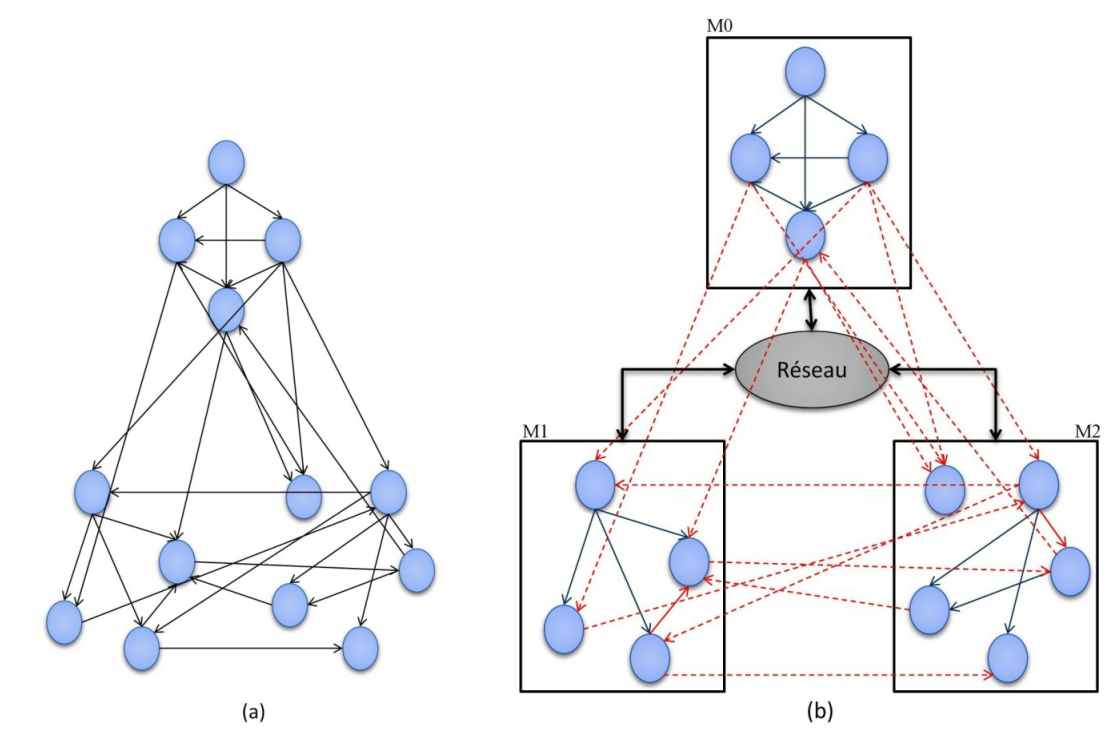
\includegraphics[height=3in]{img/eed.PNG}		
		\captionof{figure}{Un espace d’état et sa distribution sur un cluster de 3 machines, \citep{BENSETIRA2017}} \label{eed}
\end{center}

\subsection*{Approche de distribution des espaces d'états}
\paragraph{Distribution basée sur des fonctions}
 La plupart des solutions proposées pour la distribution des espaces d'états reposent sur l'utilisation d'une fonction de distribution qu'elle soit statique \citep{Garavel2013}ou dynamique \citep{Allmaier1997}, basée sur la structure de formalisme de spécification utilisé \citep{Ciardo1998}, \citep{BlomOrzan2005} ou guidée par des heuristiques \citep{Rodrigues2006}.
 \paragraph{Distribution basée sur la coloration}
 Cette approche consiste à introduire le concept de coloration et la relation de dominance dans les graphes pour trouver la bonne distribution des graphes L'approche proposée dans \citep{Guidoum2013} est basée sur le concept de la coloration forte stricte des graphes \citep{Bouzenada2012}. L'approche proposée est divisée en deux parties : un processus d'initialisation et un processus d'optimisation. Dans la première étape, les auteurs utilisent l'algorithme de coloration \citep{Bouzenada2012} qui assure la propriété de dominance. Les sorties de ce dernier (le nombre de couleurs dominées, ensemble de sommets colorés) sont exploitées pour répartir initialement le graphe et obtenir des parties disjointes. Ensuite le processus d'optimisation est utilisé pour trouver la bonne distribution.
 
 \paragraph{Distribution basé sur les métaheuristiques}
Récemment une nouvelle alternative de distribution des espaces d'états a été investiguée. Les approches proposées dans cette classe se basent sur l'utilisation des méthodes d'optimisation combinatoire, qui ont montré leur efficacité de résolution des problèmes dans différents domaines d'application.
 \\\\ 
Saidouni et al. \citep{Saidouni2012} proposent un nouvel algorithme de distribution inspiré de l'algorithme d'optimisation par essaims de particules. Les auteurs ont pu montrer comment les composants de la métaheuristique PSO comme le voisinage, les particules, et leurs vitesses et direction peuvent être adaptés pour la distribution des graphes sur une plateforme de N machines. L'approche fournit un bon équilibrage de charge et une réduction des connexions externes dans le réseau. Cependant, cette approche souffre du problème des états redondants.
\\\\
Une autre approche a été développée dans  \citep{TabibSaidouni2016},  \citep{Tabib2017}, où les auteurs ont proposé un algorithme génétique basé sur la loi gravitationnelle de Newton pour la distribution de graphes. La particularité de cette approche est que les espaces d'états sont codés par les diagrammes de décision binaires, et l'utilisation d'un modèle génétique en ilot qui repose sur l'exécution parallèle de plusieurs machines qui contiennent des populations de même taille avec la migration de leur m meilleurs individus chaque $n$ cycles.
\\\\
Saidouni et Bensetira \citep{BENSETIRA2017}, proposent un nouvel algorithme de distribution de l'espace d'états basée sur le comportement des systèmes. La particularité de cette approche est que les états sont analysés, ensuite, selon les informations pertinentes sur les états et leurs connexions (transitions internes et externes), ils sont redistribués selon une certaines heuristiques afin d'optimiser les performances du système. Cela se fait en définissant une bonne localité d'un état comme celle qui optimise à la fois l'équilibre de la charge de travail et la quantité de communication entre les machines engendrés par l'exécution de l'application opérant sur l'espace d'états distribués.